\documentclass[a4paper, ngerman]{scrartcl}
\usepackage{babel}
\usepackage{geometry}
\usepackage{graphicx}
\usepackage{fontspec}
%\usepackage{helvet}
\renewcommand{\familydefault}{\sfdefault}
%\setmainfont{Liberation Sans}
%\setsansfont{Liberation Sans}

\begin{document}
\title{Ampelsteuerung VfL Wetzlar}
\author{Peter Turczak}
\date{2020-02-02}

\maketitle
\tableofcontents
\clearpage
\section{Allgemeines}
Die durch Mitglieder des VfL Wetzlar hergestellte Ampelanlage dient zum Sperrung des "Schleusenweges" während des Flugbetriebs.

Die Anlage besteht aus zwei Verkehrsampeln, welche über W-LAN mit einander verbunden und synchronisiert werden. Eine Ampel stellt dabei den "Master" da, die "Slave"-Ampel folgt der vorgenannten in ihrem Status.

\begin{figure}
	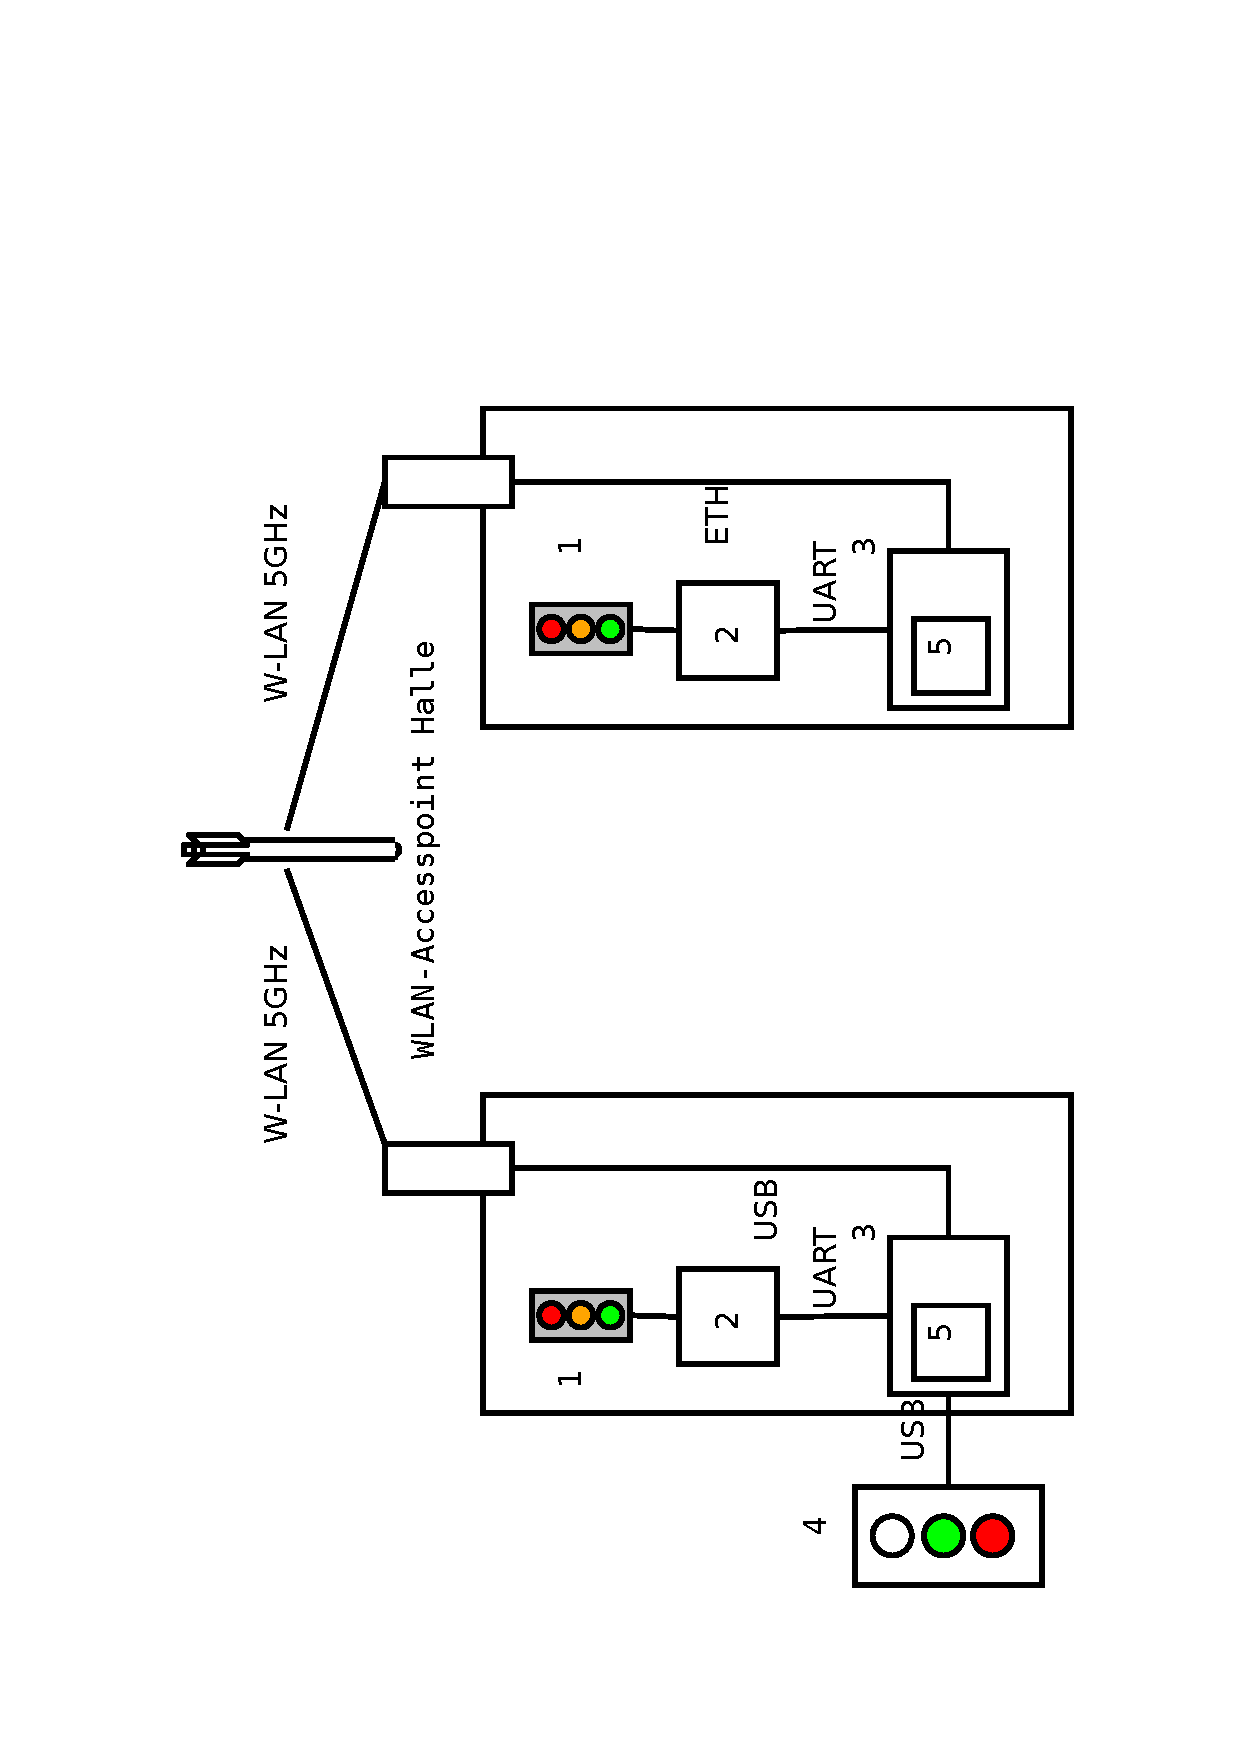
\includegraphics[keepaspectratio, width=.7\textwidth, angle=270]{Ampel_Uebersicht.pdf}
	\caption{Systemübersicht (1)~Verkehrsampel, (2)~Steuerungsplatine, (3)~Raspberry PI, (4)~Bedieneinheit, (5)~Steuerungssoftware}
\end{figure}

\section{Technische Beschreibung}
\subsection{Sicherheitskonzept}
Das Sicherheitskonzept ist in zwei Schichten ausgeführt. So wird auf elektronischer Ebene bereits eine Plausibitätsprüfung des Leuchtmittel-Zustands durchgeführt. Die festen Muster (Rot, Rot-Gelb, Grün, Gelb und Gelb blinkend) werden durch die Hardware vorgegeben und können nur in definierten Abfolgen geschaltet werden.

In der Software-Schicht wird die Synchronisierung beider Ampeln realisiert. Diese enthält Maßnahmen die z.B. eine Unterbrechung der Verbindung zwischen den Geräten möglichst sicher handhabt.
\subsection{Elektronik}
Die Steuerung der Ampel und ihrer Leuchtmittel wird über eine eigens entwickelte Leiterplatte realisiert. Diese benutzt einen PIC 16F690 für die logischen Abläufe.

Vorteil dieser Lösung ist es, dass das Programm des Mikrocontrollers bewusst nicht über den Raspberry PI verändert werden kann. Somit wird verhindert, dass persistente Malware den Ablauf auf Hardware-Ebene verändern kann. Daher wird der PIC und sein Programm von hier ab als unveränderliche Hardware betrachtet.

Um sicherzustellen, dass zu jedem Zeitpunkt die richtigen Leuchtmittel aktiv sind bzw. nicht aktiv sind, wird nicht nur die Versorgungsspannung der Leuchtmittel geschaltet. Sondern auch der Strom durch dies wird jederzeit überwacht. Hiermit können unter anderem fehlende/defekte LED-Einsätze gefunden werden, Kurzschlüsse und Verkabelungsfehler erkannt werden. Im PIC sind folgende Parameter für die Stromüberwachung vorhanden:
\begin{enumerate}
	\item Mindeststrom bei eingeschaltetem Leuchtmittel
	\item Maximalstrom bei eingeschaltetem Leuchtmittel
	\item Maximalstrom bei ausgeschaltetem Leuchtmittel
\end{enumerate}
Letzterer wird primär zum Erkennen von Kurzschlüssen und Kriechströmen verwendet.

Sollte der Strom eines Leuchmittels außerhalb der genannten Grenzen liegen, so geht die Hardware in einen Fehlerzustand, in dem die gelbe Lampe langsam blinkt, also mit einer An- und Aus-Zeit von zwei Sekunden.

Ein Fehlerzustand der Hardware kann nur durch einen Hardware-Reset, d.H. aus- und einschalten bzw. ein digitales Signal vom Raspberry PI-Prozessor zum PIC, beendet werden.

\begin{figure}
	
\includegraphics[keepaspectratio, width=\textwidth]{../pic/ampel.pdf}
	\caption{Statusübersicht der Hardware}
\end{figure}

\subsection{Sofware}
Die Software im Raspberry PI hat die Aufgabe, die beiden Ampeln mit einander zu synchronisieren. Hierbei gibt es im Grunde zwei Zustände:
\begin{itemize}
	\item Weg offen:\\
		Die Ampel sollten Grün zeigen
	\item Weg gesperrt:\\
		Beide sollten Rot anzeigen
\end{itemize}

Beide Ampeln benutzen das HTTP-Protokoll um sich mit einander zu synchonisieren, indem jeweils der Status der jeweils anderen abgefragt wird. Um Fälschungen von Statuspaketen zu erschweren, wird zwischen allen Teilnehmer ein sogenannter Group-Key abgelegt. Mit dessen Hilfe werden die Prüf-Hashes (Kryptographisch sichere Prüfsummen) vermischt, sodass Außenstehende die Pakete nicht fälschen können.

Der Zustand der als "Master" bezeichneten Ampel wird von der als "Slave" bezeichneten Ampel verfolgt. 

Sollte die Synchronisation wegen fehlender Verbindung nicht funktionieren, so versuchen beide Teilnehmer weiterhin eine Verbindung aufzubauen. Hierbei kommt es auf den Zustand des Systems an, wie darauf reagiert wird.

Ist der Weg gesperrt, so bleiben beide Ampeln rot. War der Weg freigegeben, so blinken die Ampel solange gelb, bis sie wieder synchron ist. So wird sichergestellt, dass im Zweifel lieber der Weg gesperrt wird.

\begin{figure}
	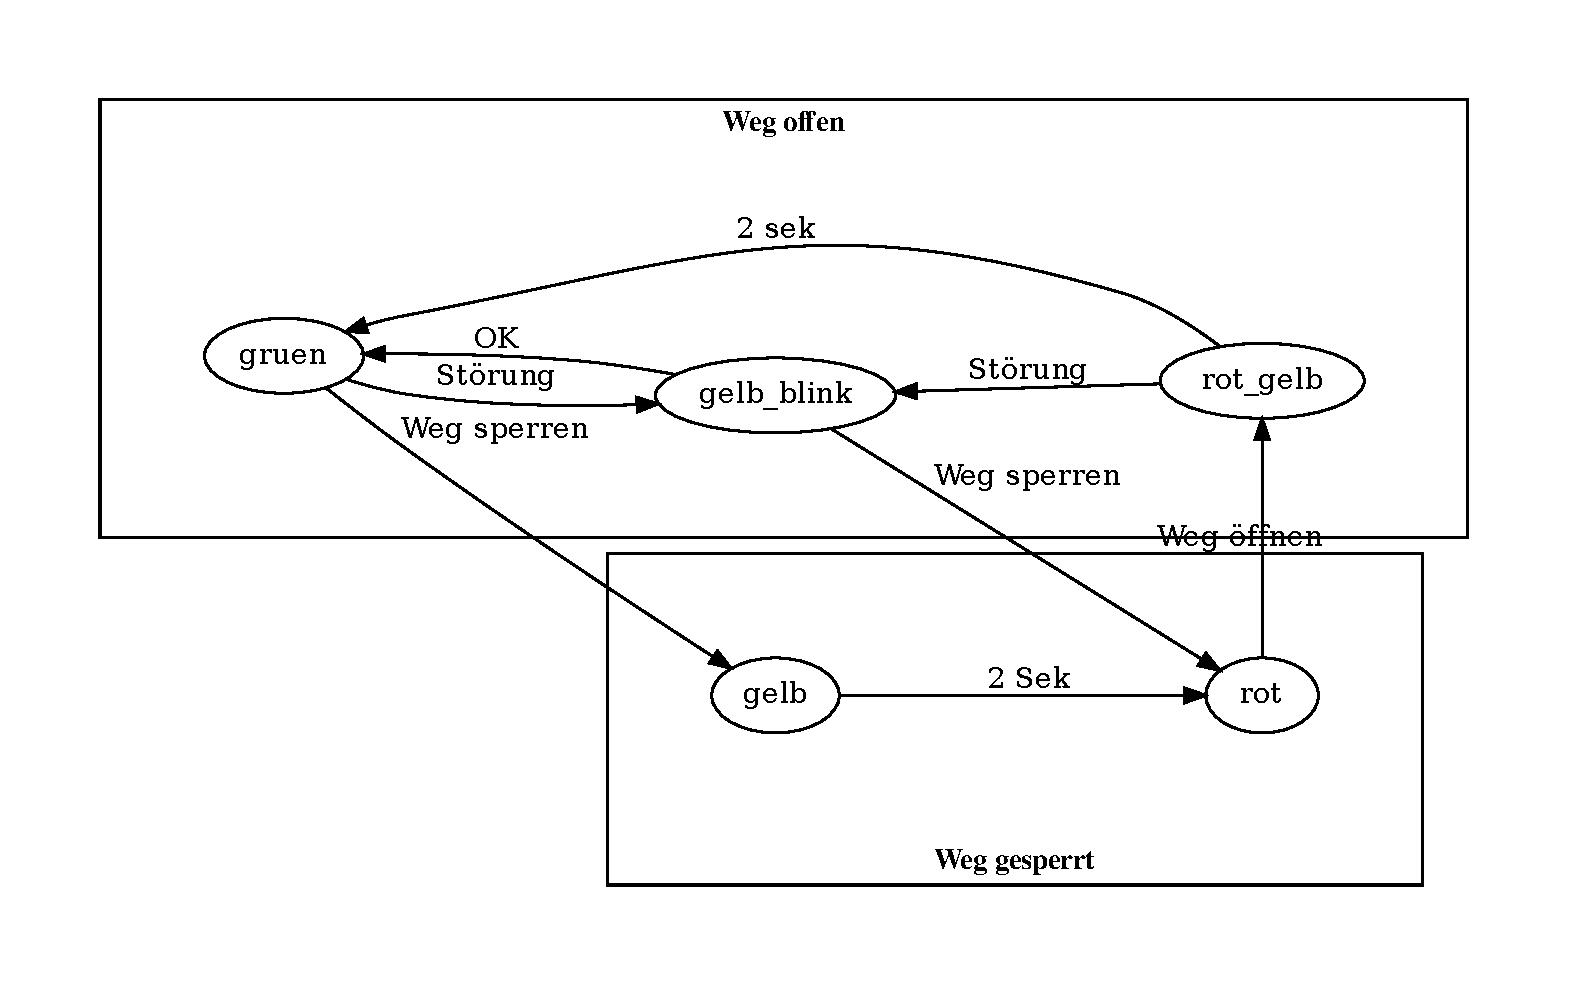
\includegraphics[keepaspectratio, width=\textwidth]{system_statemachine.pdf}
	\caption{Statusübersicht der Software}
\end{figure}

\section{Benutzung}
\subsection{Aufstellen}
Die beiden Ampeln werden zu ihren jeweiligen Aufstellorten entlang des Schleusenwegs gefahren, deren genaue Lage ist in der Flugplatzgenehmigung ersichtlich.

Ein Verankern in Boden ist gegenwärtig nicht vorgesehen, also muss auf sicheren Stand geachtet werden. Die "Master"-Ampel wird auf der Hallenseite des Schleusenweges abgestellt, die Slave-Ampel in Richung Garbenheim. Beide können auch schon von dem Aufstellen eingeschaltet werden, müssen allerdings spätestens eingeschaltet werden, wenn sie an ihrem Standort aufgestellt wurden.

Um ein Ausschalten durch Dritte zu verhindern, können die Hauptschalter beispielsweise mittels einer Fokkernadel oder eines Vorhängeschlosses im "Ein"-Zustand arretiert werden.

Nach dem Einschalten sollten die Ampeln zunächst einen Lampentest durchführen, d.H. von Rot aus werden alle Lampen für jeweils zwei Sekunden eingeschaltet und dann die nächste dazu genommen. Somit sollten dann kurzfristig alle Lampen leuchten. Wenn hierbei ein Fehler auftritt, blinkt die Betroffene Ampel langsam (jeweils zwei Sekunden ein und aus).

Das Bedienteil sollte spätestens zum Flugbetriebsbeginn eingesteckt werden, hier sollte innerhalb weniger Sekunden der Status beider Ampeln sichtbar sein.

Während der Synchronisation der Ampeln blinken beide gelb schnell (je eine Sekunde ein und aus). Sobald die erste Synchronisierung nach dem Einschalten abgeschlossen ist, sollten beide Grün zeigen.

\subsection{Sperren/Freigeben des Weges}
Der Weg kann auf zwei Arten freigegeben bzw. gesperrt werden.

Im Normalfall kann dies mit dem Bedienteil erfolgen. Durch Druck auf den roten Taster wird der Weg gesperrt, d.H. die Ampeln schalten auf Rot.  Sobald das Bedienteil auf beiden Ampeln rot zeigt, sind auch beide Ampeln sicher rot. Dies wird durch die regelmäßige Synchronisierung sichergestellt.

Ein Druck auf den grünen Taster gibt den Weg frei, d.H. die Ampeln schalten auf Grün.

Alternativ kann das Ampelsystem auch über eine Webschnittstelle vom Start aus gesteuert werden, hierzu muss der "Gruppenschlüssel" eingegeben werden. Auch dies soll verhindern, dass unberechtigte Dritte die Ampeln beeinflussen können. Diese Oberfläche ist noch in der Entwicklung daher relativ wenig intuitiv. Dies soll in den nächsten Versionen geändert werden.

\subsection{Abbau}
Am Ende des Flugbetriebs können die Ampeln einfach an deren Hauptschaltern abgeschaltet werden.

\subsection{Lagerung}
Nach dem Einräumen in die Halle sind die Ampeln aufzuladen! Hierzu werden spezielle Kabel mit dem sogenannten "Powercon"-Stecker verwendet. Es stehen zwei Stück zur Verfügung. Die Batterien sind nicht darauf ausgelegt, mehrere Tage hintereinander nur entladen zu werden!

\section{Wartung}
\subsection{Hardware}
\subsection{Software}

\section{Anhang}
\end{document}
